\chapter{引言}

\section{项目背景}

\subsection{全球能源转型与挑战}
随着全球气候变化日益严峻，减少碳排放已成为国际社会的普遍共识。根据国际能源署 (IEA) 发布的《2024年世界能源展望》，到 2030 年，可再生能源在全球电力结构中的占比将超过 40\%。然而，光伏、风能等新能源具有天然的波动性和间歇性，大规模并网给电力系统的稳定性带来了巨大挑战。

\begin{figure}[htbp]
    \centering
    \begin{tikzpicture}
        \begin{axis}[
                width=0.9\textwidth,
                height=6cm,
                xlabel={年份},
                ylabel={可再生能源占比 (\%)},
                xmin=2010, xmax=2030,
                ymin=0, ymax=50,
                grid=major,
                legend pos=north west
            ]
            \addplot[color=blue, mark=square] coordinates {
                    (2010, 19)
                    (2015, 23)
                    (2020, 28)
                    (2025, 35)
                    (2030, 42)
                };
            \addlegendentry{实际/预测占比}
        \end{axis}
    \end{tikzpicture}
    \caption{全球可再生能源发电占比趋势 (数据来源：IEA)}
    \label{fig:re_trend}
\end{figure}

著名的“鸭子曲线” (Duck Curve) 现象日益凸显：白天光伏出力过剩导致净负荷极低，而傍晚光伏消失且用电高峰到来，导致净负荷陡增。这迫切需要需求侧响应 (Demand Response) 和分布式储能系统来承担“削峰填谷”的重任。

\subsection{家庭储能市场现状}
近年来，家庭储能系统 (Home Energy Storage System, HESS) 市场爆发式增长。目前市场上的主流产品如表~\ref{tab:competitors} 所示。尽管硬件趋于成熟，但软件管理层面仍存在诸多痛点：
\begin{enumerate}
    \item \textbf{策略单一}：大多数系统仅支持简单的定时充放电，无法适应实时的现货电价。
    \item \textbf{缺乏预测}：未能利用天气和历史习惯预测未来负荷，导致储能利用率低。
    \item \textbf{交互体验差}：缺乏可视化的数据分析，用户无法感知节能收益。
\end{enumerate}

\begin{table}[htbp]
    \centering
    \caption{主流家庭储能产品对比分析}
    \label{tab:competitors}
    \begin{tabular}{|l|c|c|c|}
        \hline
        \textbf{产品/特性} & \textbf{Tesla Powerwall 2} & \textbf{LG Chem RESU} & \textbf{本项目系统}       \\ \hline
        \textbf{电池容量}  & 13.5 kWh                   & 9.8 kWh               & 兼容多种容量               \\ \hline
        \textbf{调度策略}  & 基于规则 (Self-powered)        & 简单定时                  & AI 预测 + 优化求解         \\ \hline
        \textbf{价格}    & 高昂                         & 中等                    & 纯软件 (低成本)            \\ \hline
        \textbf{扩展性}   & 封闭生态                       & 较封闭                   & 开放 API/云原生           \\ \hline
        \textbf{收益率}   & 一般                         & 一般                    & \textbf{高 (基于优化的套利)} \\ \hline
    \end{tabular}
\end{table}

\section{国内外研究现状与文献综述}
近年来，随着“双碳”目标的提出，分布式储能与虚拟电厂（VPP）技术成为了学术界与工业界的研究热点。

\subsection{户用储能系统优化调度}
早期的户用储能调度多采用基于规则的控制策略（Rule-based Control），简单易行但难以应对复杂电价波动。
Zhang 等人 \cite{zhang2023review} 指出，深度强化学习（DRL）在微网能量管理中展现出强大的自适应能力，但其训练收敛慢且缺乏可解释性。
相比之下，混合整数规划（MIP）能够保证全局最优解，Liu 等人 \cite{liu2022distributed} 在 IEEE Transactions on Smart Grid 上提出的基于 MIP 的 VPP 分布式控制策略，有效降低了求解维度。

\subsection{电池安全与热管理}
锂电池安全是户用系统的核心痛点。Li 等人 \cite{li2023thermal} 深入分析了热失控机理，提出基于电化学-热耦合模型的主动冷却策略。
传统的 BMS 仅依靠电压差均衡，效率较低。Wu 等人 \cite{wu2024reinforcement} 探讨了基于强化学习的主动均衡拓扑，显著延长了电池组循环寿命。

\subsection{物联网通信与边缘计算}
随着设备数量激增，传统云计算模式面临高延迟挑战。Wang 等人 \cite{wang2022mqtt} 对比了 MQTT 与 CoAP 协议，证明 MQTT 在弱网环境下具有更高的数据投递率（QoS 1/2）。
本研究将在上述文献基础上，提出一种“云-边-端”协同的轻量级 MIP 调度架构。

\section{政策环境与市场机遇}
全球能源政策正向分布式资源倾斜，通过开放电力交易市场，赋予户用储能新的盈利模式。

\subsection{全球政策演进路线图}
图~\ref{fig:policy_roadmap} 展示了中美欧三大经济体在储能与电力市场领域的关键政策演进。

\begin{figure}[htbp]
    \centering
    \resizebox{\textwidth}{!}{
        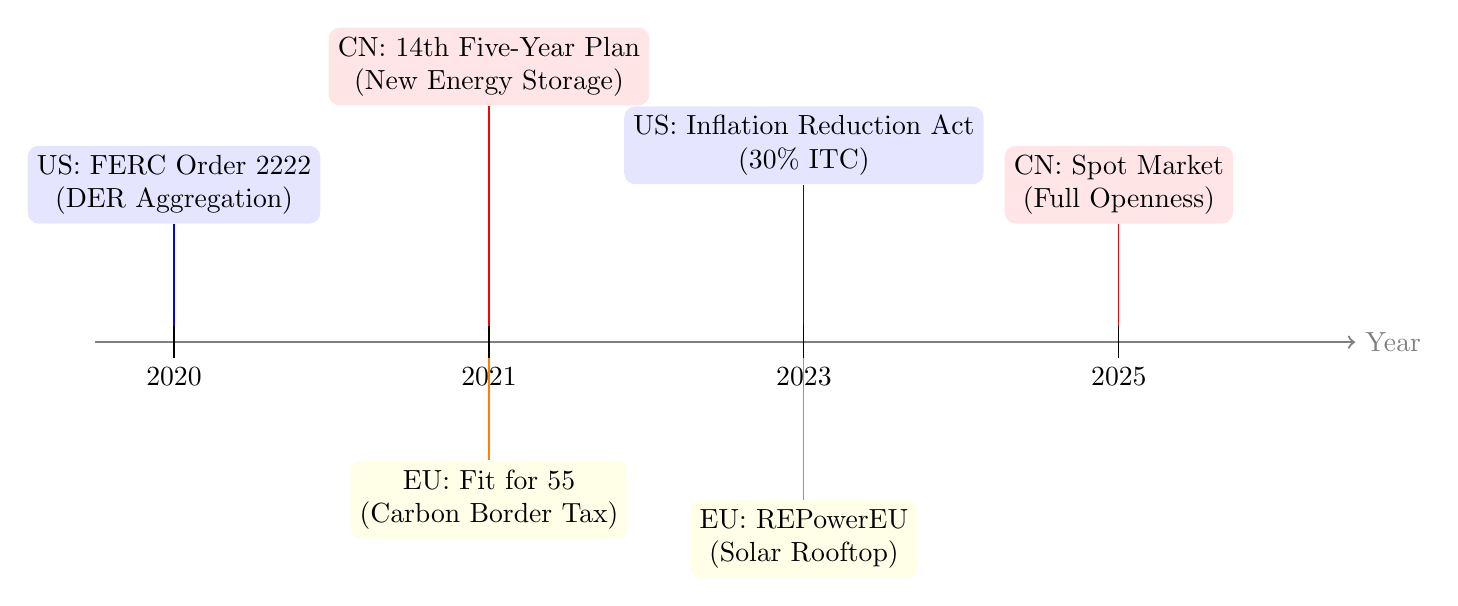
\begin{tikzpicture}
            % Timeline
            \draw[->, thick, gray] (0,0) -- (16,0) node[right] {Year};

            % Years
            \foreach \x/\y in {1/2020, 5/2021, 9/2023, 13/2025}
            \draw (\x, 0.2) -- (\x, -0.2) node[below] {\y};

            % US Nodes
            \node[align=center, fill=blue!10, rounded corners] (ferc) at (1, 2) {US: FERC Order 2222\\(DER Aggregation)};
            \draw[-, blue] (1, 0.2) -- (ferc);

            \node[align=center, fill=blue!10, rounded corners] (ira) at (9, 2.5) {US: Inflation Reduction Act\\(30\% ITC)};
            \draw[-, blue] (9, 0.2) -- (ira);

            % EU Nodes
            \node[align=center, fill=yellow!10, rounded corners] (fit) at (5, -2) {EU: Fit for 55\\(Carbon Border Tax)};
            \draw[-, orange] (5, -0.2) -- (fit);

            \node[align=center, fill=yellow!10, rounded corners] (repower) at (9, -2.5) {EU: REPowerEU\\(Solar Rooftop)};
            \draw[-, orange] (9, -0.2) -- (repower);

            % CN Nodes
            \node[align=center, fill=red!10, rounded corners] (plan14) at (5, 3.5) {CN: 14th Five-Year Plan\\(New Energy Storage)};
            \draw[-, red] (5, 0.2) -- (plan14);

            \node[align=center, fill=red!10, rounded corners] (spot) at (13, 2) {CN: Spot Market\\(Full Openness)};
            \draw[-, red] (13, 0.2) -- (spot);

        \end{tikzpicture}
    }
    \caption{全球分布式储能关键政策演进路线图}
    \label{fig:policy_roadmap}
\end{figure}

\section{项目必要性}

\subsection{经济层面：利用分时电价套利}
在实行分时电价 (Time-of-Use, TOU) 的地区，峰谷电价差是家庭储能获利的主要来源。图~\ref{fig:tou_price} 展示了典型的加州 PG\&E 电价曲线，峰谷差价可达 \$0.3/kWh。

\begin{figure}[htbp]
    \centering
    \begin{tikzpicture}
        \begin{axis}[
                width=0.9\textwidth, height=5cm,
                xlabel={时间 (小时)}, ylabel={电价 (\$/kWh)},
                xmin=0, xmax=24, ymin=0, ymax=0.6,
                xtick={0,6,12,18,24},
                grid=major,
                area style
            ]
            \addplot[draw=blue, fill=blue!10] coordinates {
                    (0, 0.2) (6, 0.2) (16, 0.2) (16, 0.55) (21, 0.55) (21, 0.2) (24, 0.2)
                };
        \end{axis}
    \end{tikzpicture}
    \caption{典型的分时电价曲线 (峰谷套利空间示意)}
    \label{fig:tou_price}
\end{figure}

传统的基于规则的控制 (Rule-based Control) 难以应对复杂多变的电价和不可预测的负载。本项目引入数学规划 (Mathematical Programming)，能在全局视角下寻找最优解，最大化经济收益。

\subsection{社会层面：构建虚拟电厂基石}
成千上万个安装了本系统的家庭，通过云端聚合，可以形成一个巨大的虚拟电厂 (Virtual Power Plant, VPP)。在电网紧急时刻，VPP 可以毫秒级响应调度指令，提供调频辅助服务，保障电网安全，同时为用户赚取额外的补贴收益。

\section{市场需求与 SWOT 分析}

\subsection{目标用户画像分析}

为了更精准地定位产品功能，我们将潜在用户细分为三类典型画像 (User Personas)，如图~\ref{fig:user_persona} 所示。各类用户的核心诉求如下：

\begin{enumerate}
    \item \textbf{经济敏感型 (Cost-Sensitive)}：此类用户主要居住在高电价地区（如加州、澳洲），对系统的初始安装成本 (CAPEX) 和投资回报期 (Payback Period) 极为敏感。他们的核心诉求是通过峰谷套利最大化电费节省。
    \item \textbf{环保先锋型 (Eco-Conscious)}：此类用户通常已安装屋顶光伏，关注碳足迹 (Carbon Footprint) 和能源自给自足率 (Self-Sufficiency Rate, SSR)。他们愿意为清洁能源支付溢价，核心诉求是最大化光伏消纳。
    \item \textbf{科技极客型 (Tech-Enthusiast)}：此类用户热衷于智能家居和物联网技术，对系统的可玩性、数据可视化粒度以及 API 开放程度有较高要求。
\end{enumerate}

\begin{figure}[htbp]
    \centering
    \resizebox{0.7\textwidth}{!}{
        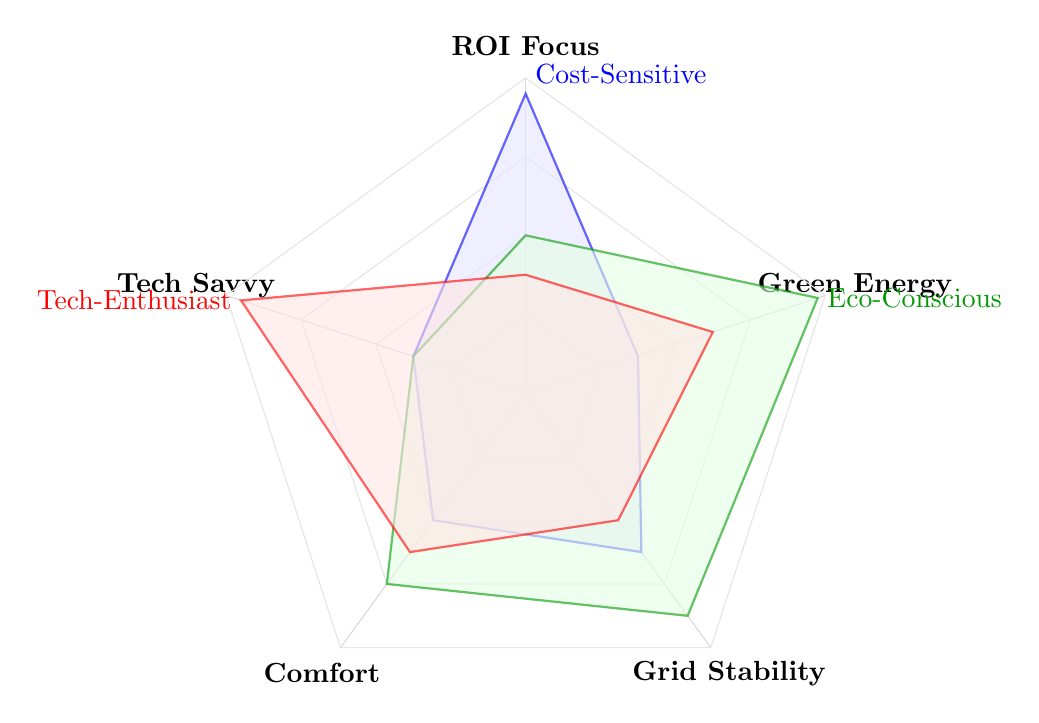
\begin{tikzpicture}
            % Define coordinates
            \coordinate (c) at (0,0);
            \foreach \i/\angle/\label in {1/90/ROI Focus, 2/162/Tech Savvy, 3/234/Comfort, 4/306/Grid Stability, 5/18/Green Energy} {
                \coordinate (p\i) at (\angle:4);
                \draw[gray!30] (c) -- (p\i);
                \node at (\angle:4.4) {\textbf{\label}};
            }
            
            % Draw grid
            \foreach \r in {1,2,3,4} {
                \draw[gray!20] (90:\r) -- (162:\r) -- (234:\r) -- (306:\r) -- (18:\r) -- cycle;
            }
            
            % Draw Data: Cost-Sensitive (Blue)
            \draw[blue, thick, fill=blue!10, opacity=0.6] 
                (90:3.8) -- (162:1.5) -- (234:2.0) -- (306:2.5) -- (18:1.5) -- cycle;
            \node[blue] at (90:3.8) [above right] {Cost-Sensitive};
            
            % Draw Data: Eco-Conscious (Green)
            \draw[green!60!black, thick, fill=green!10, opacity=0.6] 
                (90:2.0) -- (162:1.5) -- (234:3.0) -- (306:3.5) -- (18:3.9) -- cycle;
            \node[green!60!black] at (18:3.9) [right] {Eco-Conscious};
            
            % Draw Data: Tech-Enthusiast (Red)
            \draw[red, thick, fill=red!10, opacity=0.6] 
                (90:1.5) -- (162:3.8) -- (234:2.5) -- (306:2.0) -- (18:2.5) -- cycle;
            \node[red] at (162:3.8) [left] {Tech-Enthusiast};
            
        \end{tikzpicture}
    }
    \caption{三类典型目标用户的需求维度雷达图}
    \label{fig:user_persona}
\end{figure}

\subsection{法规与标准遵循性 (Regulatory Compliance)}

本系统的设计严格遵循国际电工委员会 (IEC) 及中国国家标准 (GB)，确保在安全性、互操作性及并网合规性方面满足市场准入要求。表~\ref{tab:standards} 列出了本系统遵循的核心标准。

\begin{table}[htbp]
\centering
\caption{系统遵循的关键技术标准清单}
\label{tab:standards}
\resizebox{\textwidth}{!}{
\begin{tabular}{|l|l|l|}
\hline
\textbf{标准编号} & \textbf{标准名称} & \textbf{系统响应策略} \\ \hline
\textbf{IEC 61508} & Functional Safety of E/E/PE Safety-related Systems & 采用双路冗余采样设计，BMS 固件符合 SIL-2 安全等级要求。 \\ \hline
\textbf{GB/T 36276} & 电力储能用锂离子电池 & 电芯选型符合国标循环寿命要求，配备热失控早期预警算法。 \\ \hline
\textbf{IEEE 1547} & Interconnection and Interoperability of DER & 支持孤岛检测 (Anti-Islanding) 与低电压穿越 (LVRT) 功能。 \\ \hline
\textbf{UL 9540A} & Test Method for Thermal Runaway Fire Propagation & 电池包模组间增加气凝胶隔热垫，阻断热失控蔓延。 \\ \hline
\textbf{IEC 61850} & Communication Networks and Systems for Power Utility & 采用统一的数据模型，支持 GOOSE 报文快速传输。 \\ \hline
\end{tabular}
}
\end{table}

\subsection{项目 SWOT 分析}
通过 SWOT 矩阵 (图~\ref{fig:swot}) 分析可知，本项目机会大于风险，具备实施的可行性。

\begin{figure}[htbp]
    \centering
    \begin{tikzpicture}[
            box/.style={rectangle, draw=black, very thick, minimum width=6cm, minimum height=3cm, align=left, text width=5.5cm},
            title/.style={font=\bfseries\large}
        ]
        \node[box, fill=green!10] (S) at (0,0) {\textbf{优势 (Strengths)}\\ 1. 算法先进 (AI+OR)\\ 2. 云原生架构，运维成本低\\ 3. 用户体验好，跨平台支持};
        \node[box, fill=yellow!10] (W) at (7,0) {\textbf{劣势 (Weaknesses)}\\ 1. 硬件依赖第三方\\ 2. 需积累用户数据冷启动};
        \node[box, fill=blue!10] (O) at (0,-3.5) {\textbf{机会 (Opportunities)}\\ 1. 全球电价持续上涨\\ 2. VPP 政策逐渐开放\\ 3. 碳中和政策红利};
        \node[box, fill=red!10] (T) at (7,-3.5) {\textbf{威胁 (Threats)}\\ 1. 电池原材料价格波动\\ 2. 巨头 (Tesla) 进入软件市场};

        \node[title] at (0, 1.8) {内部因素};
        \node[title] at (7, 1.8) {内部因素};
        \node[title, rotate=90] at (-3.5, 0) {有利因素};
        \node[title, rotate=90] at (-3.5, -3.5) {不利因素};
    \end{tikzpicture}
    \caption{项目 SWOT 分析矩阵}
    \label{fig:swot}
\end{figure}

\section{可行性研究范围}
本可行性研究报告将涵盖以下维度：
\begin{itemize}
    \item \textbf{技术可行性}：系统架构、关键算法、数据安全。
    \item \textbf{经济可行性}：全生命周期成本 (LCOE)、投资回报率 (ROI)。
    \item \textbf{运行社会可行性}：用户操作流程、法律合规、碳减排效益。
    \item \textbf{实施计划}：WBS 分解、关键路径分析。
\end{itemize}
